%% Overleaf			
%% Software Manual and Technical Document Template	
%% 									
%% This provides an example of a software manual created in Overleaf.

\documentclass{ol-softwaremanual}

% Packages used in this example
\usepackage{graphicx}  % for including images
\usepackage{microtype} % for typographical enhancements
\usepackage{minted}    % for code listings
\usepackage{amsmath}   % for equations and mathematics
\setminted{style=friendly,fontsize=\small}
\renewcommand{\listoflistingscaption}{List of Code Listings}
\usepackage{hyperref}  % for hyperlinks
\usepackage[a4paper,top=4.2cm,bottom=4.2cm,left=3.5cm,right=3.5cm]{geometry} % for setting page size and margins
\usepackage{helvet}
\usepackage{dirtree}
\renewcommand{\familydefault}{\sfdefault}


% Custom macros used in this example document
\newcommand{\doclink}[2]{\href{#1}{#2}\footnote{\url{#1}}}
\newcommand{\cs}[1]{\texttt{\textbackslash #1}}

% Frontmatter data; appears on title page
\title{\Huge \mdseries \textbf{Lumen Data Science 2023} \\ Harmony Is All You Need \\ \Large Technical documentation}
\version{1.0}
\author{Tin Ferković, Dorian Smoljan \\ \normalsize University of Zagreb}
\softwarelogo{
\includegraphics[width=8cm]{images/lumen.png}}

\begin{document}

\maketitle

\tableofcontents
\listoflistings
\newpage

\section{Introduction}

The goal of this technical documentation is to describe the technical implementation of the solution developed by our team as a part of the Lumen Data Science 2023 competition, on the subject of instrument and human voice detection in audio files.

\clearpage

\section{Project structure and organization}

This section describes the structure of our project, including the technologies and tools used, directory structure, and experiments setup and tracking.


\subsection{Languages and libraries}

We used a number of software tools to develop our solution. As a programming language we, of course, used Python, alongside Conda as a package manager. To load, analyze and transform audio files we used Librosa, a Python library for music and audio analysis which proved exceptionally powerful and simple to use. For data analysis, Pandas came in handy, alongside Matplotlib and its wrapper, Seaborn.

As for the implementation of our deep learning models, which made up the majority of the models we experimented with, we first tried using plain PyTorch, but soon decided to switch to PyTorch Lightning, a high-level wrapper around PyTorch. It allowed us to better organize our code, reduce boilerplate and implement new models faster. It was the first time either of us worked with Lightning, and we were pleasantly surprised by the ease of setup and the improvements it brought, and we plan to keep using it in our future experiments.

To develop an application to showcase our solution, we used \doclink{https://fastapi.tiangolo.com/}{FastAPI}  for backend, and \doclink{https://streamlit.io/}{Streamlit} for frontend. We also used \doclink{https://www.docker.com/}{Docker} to containerize our application and enable it to be run virtually anywhere by using a single command. 


\subsection{Code structure and organization}
One very important, but sometimes overlooked key to good projects is their
structure. If badly structured, no matter how good the project’s idea or implementation is, it is more likely to fail than to succeed. With that in mind, we
paid special attention to the structure and organization of our project. \\


In order to achieve this, several things were done. Firstly, we followed PyTorch Lightning's guidelines and extracted every model architecture we developed into its own Lightning Module, while the logic common to all models (train and evaluation loop, optimizer configuration, and logging) was extracted to a single module. This module would then be able to take any of our model architectures and use them for training/evaluation, increasing the modality and decoupling our code. It also meant that, if we wanted to experiment with a new model architecture, all we had to do was to define it in its own module and inject it into the base module, which would take care of the training/evaluation. \\

Secondly, as we run a lot of different experiments using a plethora of different models, we needed to constantly manage a lot of configuration, as each model or experiment required some different parameters in order to achieve the best results. In order to be able to do this in an organized way, we used \doclink{https://hydra.cc/docs/intro/}{Hydra}, a Python library for configuration handling. This enabled us to split every part of our configuration into a separate .yaml file, which could then be easily altered or exchanged for a different configuration file to achieve different behavior. For example, we could define one configuration file for training a ResNet model, complete with definitions for its specific learning rate and optimizers, and another for the audio transformer model, with different hyperparameters. Then, once we have these two different configs, experimenting with different models is just a matter of referencing a different model config file in the master configuration file. An example of a Hyrdra .yaml configuration file can be seen in Listing 1. Furthermore, Hydra also supports object instantiation, which meant that everything we need to define an experiment could be setup and instantiated directly for Hydra, eliminating the need for changing configurations and parameters in 10 different files each time a new experiment is run. \\

Finally, in order to logically organize our code and configuration into proper directories and subdirectories, we used a slightly modified version of the excellent \doclink{https://github.com/ashleve/lightning-hydra-template}{Lightning-Hydra-Template}, a template for organizing deep learning projects using PyTorch Lightning and Hydra. It provided an invaluable resource for code and experiment organization, helping us efficiently organize all our components into a whole. \newline

\begin{listing}
\inputminted{yaml}{code/hydra_example.m}
\caption{Example Hydra configuration .yaml file}
\label{listing:octave}
\end{listing}

A Github project repository was used to keep track of all changes made during development. 
\subsection{Data organization}

IRMAS dataset was provided to us in a train and evaluation split; we futher split we evaluation dataset into  a validation and test datasets with the ratio 30-70. Audioset was simply split into train-val-test using the standard 70-10-20 split. The same splits were used for every model we evaluated. Each dataset and its train/test/val was referenced by a .csv file, which contained all the information required for the dataloader to load the dataset examples into memory and pass them to the training module. 

\subsection{Running and monitoring experiments}

All the experiments were run on a computer equipped with an NVIDIA RTX 2080TI GPU with 11 GB of VRAM. In order to monitor and visualize the progression of our experiments, we initially used \doclink{https://www.tensorflow.org/tensorboard}{Tensorboard}, but after a bit of research, we decided to try out \doclink{https://wandb.ai/home}{Weights\&Biases}, as neither of us had used it before and we wanted to give it a try. And we were pleasantly surprised - in general, we found it more informative and easier to use than Tensorboard, especially when comparing different experiments. It also enabled us to create a team space, where we could easily monitor all experiments, regardless on whose computer the experiment was run. An example of a Weights\&Biases experiment overview can be seen in Figure 1. \\

\begin{figure}[h]
\centering
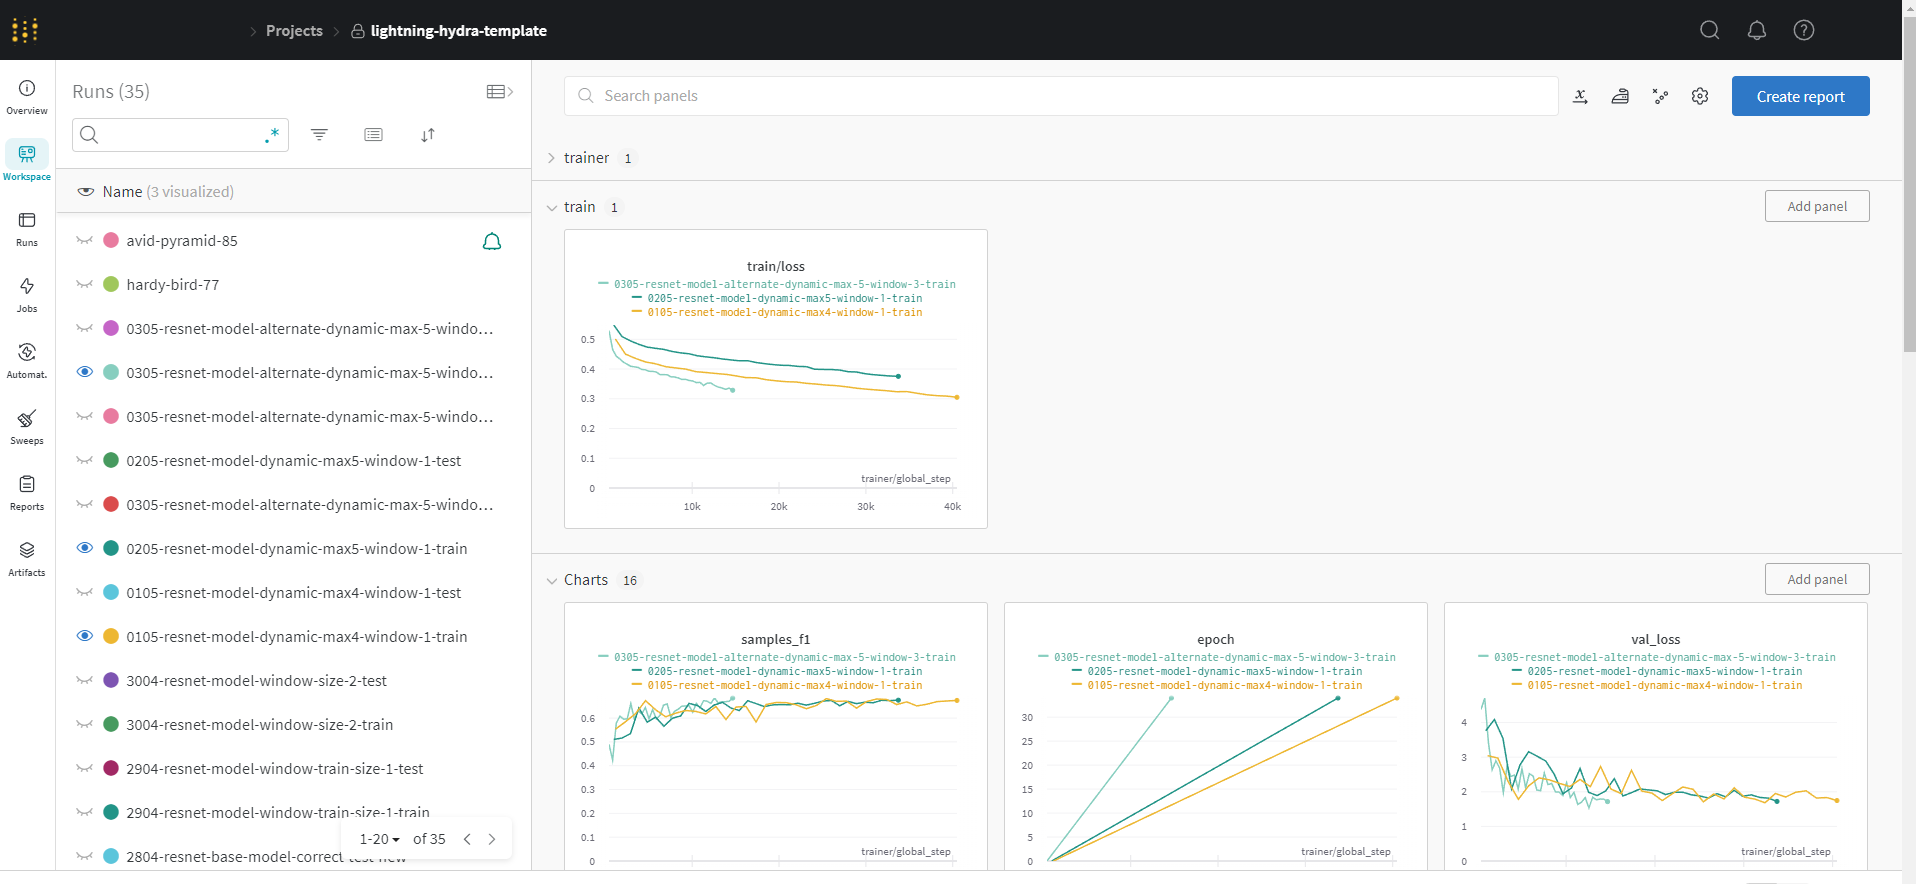
\includegraphics[width=1.0\textwidth]{images/wandb.png}
\caption{\label{fig:wandb}Weights\&Biases experiments overview}
\end{figure}


\subsection{Exporting trained models}

Once our models were trained and evaluated, we chose the best models and exported them to an archive format using \doclink{https://pytorch.org/docs/stable/jit.html}{Torchscript}. The archived model could then be easily used by the backend service in order to make predictions. We believe this is a better approach compared to using regular PyTorch checkpoints, as Torchscript exported models do not require the source code of the original model to run, while regular PyTorch checkpoint files do, thus creating a dependency between the final application and the source code of the model. Also, interestingly enough, Torchscript checkpoints are substantially smaller, for example, the checkpoint for the final model (ResNet-50), saved as a regular PyTorch .ckpt file had a size of 276MB, while the same model saved as a Torchscript checkpoint, .pt, was only 92MB in size.


\subsection{Group organization and communication}

For team communication, we used Discord, WhatsApp, and Google Meet. We also used Evernote to keep track of new ideas and take notes for the project documentation. As we already used Github for version tracking and syncing changes to our code, we also took advantage of its pull requests feature for code reviews. \clearpage

\section{Application startup and usage guide}

In this section, we will give a short description of the application we developed to showcase the functionality of our models, as well as a guide on how to set up and use the application. 

\subsection{Application startup}

There are two main ways to run the backend and frontend applications: using Docker, and running the applications as Python programs directly.

\subsubsection{Running the application using Docker}

The easiest way of starting the application is by using docker-compose, which starts both the backend and frontend by default. Simply make sure that you have Docker installed and that your Docker daemon is running, and then follow the steps described below.

\begin{enumerate}
\item Position yourself in the src/app directory
\item Run \texttt{docker-compose -f docker-compose.yml up}
\item Acess the UI on \url{localhost:8501}, or the backend API on \url{localhost:8080}
\end{enumerate}

It is also possible to run only the backend service, or only the frontend service. To do this, you can do the following: \\

\textbf{Backend service}
\begin{enumerate}
\item Position yourself in the src/app/backend directory
\item Run \texttt{"docker run --gpus=all -p 8080:8080 app\_backend"}
\item Acess the backend API on \url{localhost:8080}
\end{enumerate} \\

\textbf{Frontend service}
\begin{enumerate}
\item Position yourself in the src/app/frontend directory
\item Run \texttt{"docker run -p 8501:8501 app\_frontend"}
\item Acess the frontend app on \url{localhost:8501}
\end{enumerate}

When running an application using Docker, please make sure you have Docker installed and Docker daemon running. Furthermore, make sure you have  \doclink{https://docs.nvidia.com/datacenter/cloud-native/container-toolkit/install-guide.html}{NVIDIA Container Toolkit} installed, as it is possible that without it, Docker will not be able to recognize your NVIDIA driver. \\

Note: we ran into a couple of issues when starting our app using Docker and Docker compose, relating to the container not being able to recognize the NVIDIA driver installed on our system. The first time we set up Docker images and started the app using docker-compose.yaml, everything worked flawlessly. However, when we (purposely) deleted both images and reinstalled them, to make sure everything worked fine, we got the error described above, even though there were no changes made to the Docker files or Python scripts. We tweaked the Docker files a bit, and made sure \doclink{https://stackoverflow.com/questions/59008295/add-nvidia-runtime-to-docker-runtimes}{Docker's default runtime is NVIDIA}, and it started working again. We tested it on two different computers, one running Linux Ubuntu and one Ubuntu in WSL, and it worked, even after running \texttt{"docker system prune -a"} and reinstalling the images, but as we're still unsure what caused the original error, we are aware you might run into the same issue. If you do, you can try some of the troubleshooting steps we listed here, but if none work, you can start the applications without using Docker using steps from 3.2

\subsubsection{Running the application without using Docker}

\textbf{Frontend service}

\begin{enumerate}
\item Position yourself in the src/app/frontend directory
\item Run \texttt{"pip install -r requirements.txt"} to install all the necessary requirements for the app to run
\item Run \texttt{"streamlit run main.py"}
\item Acess the frontend app on \url{localhost:8501}
\end{enumerate}

 \noindent \textbf{Backend service}

\begin{enumerate}
\item Position yourself in the src/app/backend directory
\item Run \texttt{"pip install -r requirements.txt"} to install all the necessary requirements for the app to run
\item Run \texttt{"python main.py"}
\item Acess the backend app on \url{localhost:8080}
\end{enumerate} \\

\subsection{Using the application}

There are two main ways to use the application - through the UI, or by sending requests to the application API. In this section, we are going to give a short introduction to how to use both ways.

\subsubsection{Using the application through the UI}

If you followed the instructions from section 3.1, you should now have the backend service running on \url{localhost:8080} and the frontned service running on \url{localhost:3000}. You can go ahead and open the frontend URL in your favorite browser. Once you open it, you should see the screen shown in Figure 2. 

\begin{figure}[H]
\centering
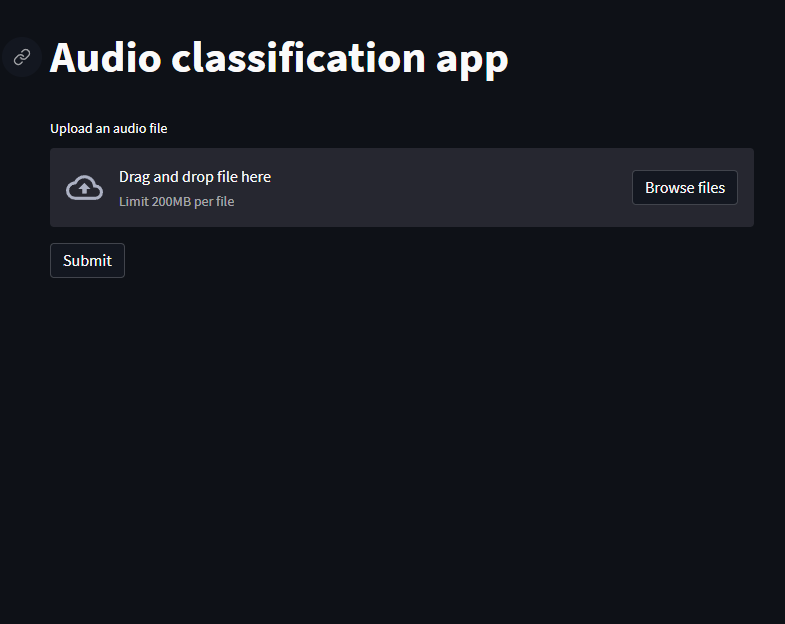
\includegraphics[width=1.0\textwidth]{images/app_1.png}
\caption{\label{fig:wandb}Initial application screen}
\end{figure}

To get a prediction, first, find an audio file you want to analyze by clicking the "Browse files" button and finding your file.\\

Now that you found your file, you can also play it to make sure it is the file you really want. If you are satisfied with the chosen file, click "Submit". The application takes a couple of seconds to make a prediction, depending mainly on whether you have a GPU on your system or not. \\

After a couple of seconds, you should see the screen shown in Figure 3, indicating which instruments were detected in your audio file!

\begin{figure}[h]
\centering
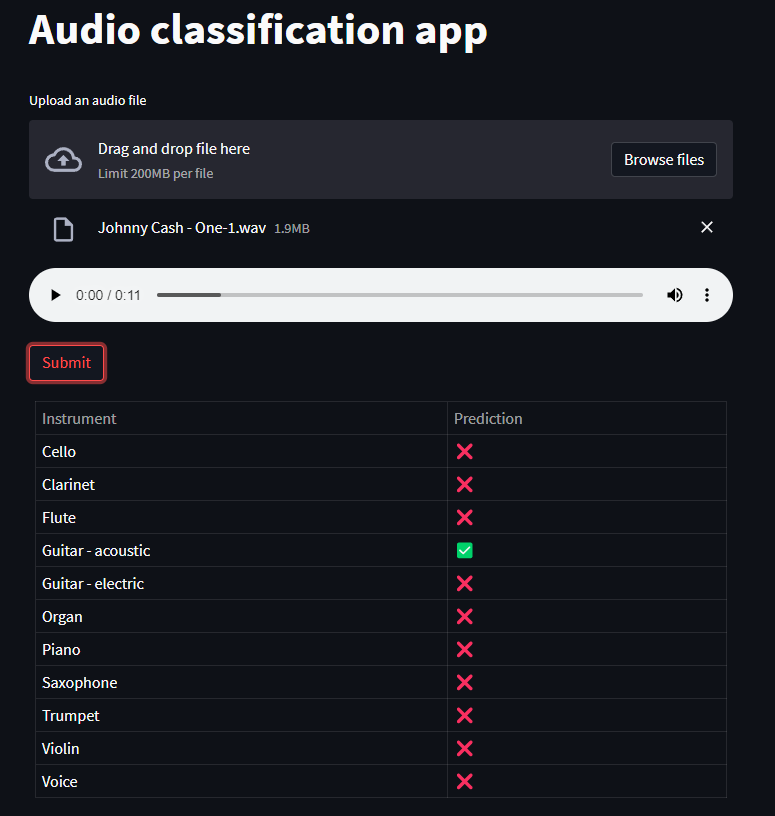
\includegraphics[width=1.0\textwidth]{images/app_2.png}
\caption{\label{fig:wandb}Screen showing the predicted instruments}
\end{figure}

\subsubsection{Using the application API}

Using the API is really simple. All you have to do is start the backend service using the steps described in section 3.1, which starts the service on \url{localhost:8080}. The prediction service is listening on the \url{/api/prediction} endpoint. This endpoint expects a single  image file, encoded as multipart form data in the incoming HTTP request.

The easiest way to test the API is through \doclink{https://www.postman.com/}{Postman}, an API platform for building and testing API's. To do so, run Postman and create a new request of type "POST", and set it's URL to the backend service URL, \url{localhost:8080/api/predict}. Then, simply fill in the fields in the "Body" section as shown in Figure 4, making sure to select the file you want to send. After that, click send, and you will soon receive the response in JSON format.\\

\begin{figure}[h]
\centering
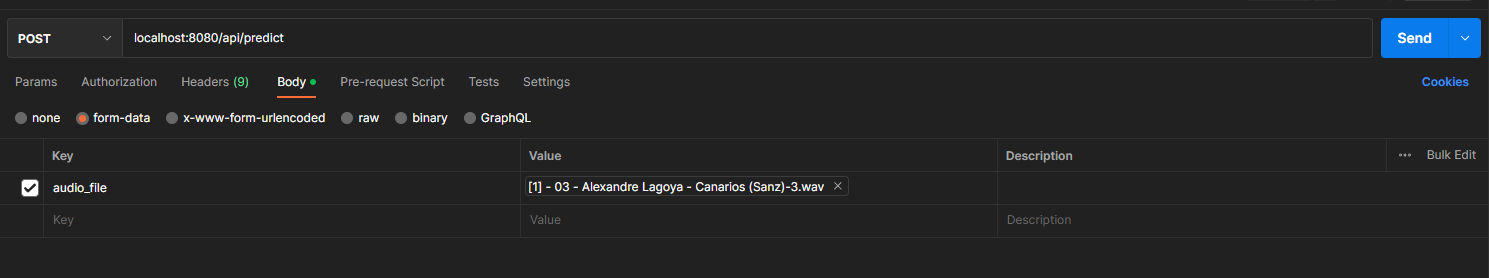
\includegraphics[width=1.0\textwidth]{images/postman_1.png}
\caption{\label{fig:wandb}Postman fields setup}
\end{figure}


\clearpage
\section{Reproduciability guide}

In this section, we will give instructions on how to setup directories and configuration if you want to replicate our results or continue training the models we developed. 

\subsection{Cloning the project}

Our source code is available at \\ \url{https://github.com/dsmoljan/Lumen-Data-Science-2023}. Simply clone our repository using Git, and open it using your favorite IDE.

\subsection{Code structure}

The cloned repository contains multiple directories, including the documentation, meeting notes, and notebooks used in our project. The code necessary for replication of our results is located in the \textit{Code} directory.

Inside the Code directory, you can find the \textit{configs} directory, containing the Hydra configuration files.

In the \textit{src\slash model} directory, you can find the code used for training and evaluating models, including the model architecture in \textit{model} package, data-related classes, such as \textit{audio\_dataset.py} in \textit{data\_utils} package, and various helper methods in the \textit{utils} package. \clearpage


\subsection{Configuration}

The main way to define which models and with which parameters to run is by configuring .yaml files in the \textit{configs} directory.  Out of these configuration files, the most important ones are \textit{train.yaml} and \textit{eval.yaml} - these are the main configuration files for training and evaluation loops, so any changes you want to make are likely going to be in these files, or by changing the sub-configuration files referenced. For example, if you added a new model and want to use it for training, you would simply define its configuration .yaml file in the \textit{configs\slash model\slash} directory, and then reference that configuration file in the field "model" in train.yaml configuration file.


Finally, you'd want to define your project root directory by modifying the appropriate variable in the .env file located in \textit{Code} directory.

\subsection{Training and evaluating models}

After you have finished setting up the configuration files to suit your experiment, make sure to create a new Conda environment containing all dependencies needed to run our project. You can do this by running the following command: \\

\noindent \textit{conda env create -n ENVNAME \--\--file PATH\_TO\_OUR\_PROJECT/src/model/environment.yml} \\

\noindent where \texttt{ENVNAME} is the name you want to give your new environment, and \texttt{PATH\_TO\_OUR\_PROJECT} full system path to the Code folder of our project. \\

You can start training by positioning yourself in the \textit{Code} directory and running the following command: \newline
\texttt{python -m src.model.train}. \newline

Similarly, if you want to evaluate a trained model, run the command: \newline \texttt{python -m src.model.eval}

\end{document}
